\title{Introduction to \myTikZ}
\author{
  Herman Jaramillo Villegas \\
  Universidad de Medell\'in
}
\date{\today}


\documentclass[12pt]{article}
\usepackage[pdftex]{graphicx}
\usepackage{amsmath}
\usepackage{hyperref}
\usepackage{pgfplots}
\usetikzlibrary{arrows.meta}
\usepackage{listings}
\usepackage{mathpazo}
\usepackage{comment}
\usepackage{alltt}
\usepackage{circuitikz}

\usepackage{tikz-3dplot}
\usetikzlibrary{decorations.markings,arrows}
\pgfplotsset{compat=newest}

\usepackage{hyperref}

\usepackage{neuralnetwork}


% Define a custom command for TikZ
\newcommand{\myTikZ}{Ti\textit{k}Z }
\newcommand{\myLaTeX}{\LaTeX \space  }

\newcommand{\myTask}{\begin{center} I need to do this many times \end{center}}

\renewcommand{\lstlistingname}{Listado}

\lstset{basicstyle=\ttfamily,
  showstringspaces=false,
  commentstyle=\color{red},
  keywordstyle=\color{blue}
}


\usepackage[a4paper, margin=2cm]{geometry} % Load geometry package and set margins




% Define a TikZ macro to draw a colored circle
\newcommand{\coloredcircle}[2]{ % Takes two arguments: color and radius
  \begin{tikzpicture}
    \fill[#1] (0,0) circle (#2);
  \end{tikzpicture}
}

\begin{document}
\maketitle

\section{Introduction}
\myTikZ is a powerful package to do graphics in a \myLaTeX environment.
It is designed to generate high-quality diagrams, figures, and illustrations. 
The package \myTikZ is part of a combination 
\href{https://en.wikipedia.org/wiki/PGF/TikZ}{PGF/\myTikZ}
\footnote{https://en.wikipedia.org/wiki/PGF/TikZ}
which are programs to create 
\href{https://en.wikipedia.org/wiki/Vector_graphics}{vector graphics.}
\footnote{https://en.wikipedia.org/wiki/Vector\_graphics}
My book in Calculus has more than 190 graphs created with \myTikZ.  I show a few of the
Figures to illustrate their quality.
%\footnote{Check this with the command 
%  \texttt{> grep begin{figure *.tex | wc}  while standing on the source repository for the
%book.}
\footnote{Check this with the command 
  \begin{alltt}
    \hspace{2in} grep begin\{figure *.tex | wc
  \end{alltt}
}

Only two of the figures in that book are not made with \myTikZ.

\myTikZ was created as complement to \myLaTeX due to the lack of tools that \myLaTeX had
for graphics. \myTikZ allows the construction of shapes, lines, curves, colors, and other
geometrical objects.  These constructions are precise due to instructions on positions
programmed for each point in the graph. The \myTikZ community has developed packages
which facilitate the work in \space \myTikZ. For example, packages on circuits, neural networks,
flowcharts, and more.

The online documentation is found  in the website
\href{https://tikz.dev/}{online documentation for \myTikZ and PGF Packages.}
\footnote{https://tikz.dev/}
or just type ``\texttt{tikz pdf manual}'', in google for example, if you want a PDF document.



\subsection{What are the advantages of using \myTikZ ?}
Here is an incomplete list of good attributes in \myTikZ.

\begin{itemize}
  \item \myTikZ has a steep learning curve, but once you get used to it you want to stay there.
    It is \textbf{flexible} and can be reused for multiple purposes.  
  \item \textbf{Integration with} \myLaTeX : This is a great advantage. 
    It allows for the edition of articles and books with high professional look.
  \item \myTikZ is
    \textbf{accurate}. Since its instructions are based on accurate metrics, the figures can be
    done with precision.  
  \item \myTikZ can help on \textbf{understanding mathematical
    problems}.  Some times we need to draw figures to understand a mathematical problem.
    Sketches help in many situations but sometimes precision is needed to have a proof of
    concept. \myTikZ is good for these tasks.  
  \item \myTikZ is  \textbf{light}. Since the
    instructions are text lines, they will not weight much; still they can generate vector
    graphics of large size. When we share work we share the source and not the figures. Moving
    and storing \myLaTeX files is easy and cheap.
  \item \textbf{Vector Graphics}: This means that the generated graphics have multiresolution
    attributes. That is they can be scaled without loosing any resolution.
  \item \textbf{Extensive Libraries}: There are, in the community, a lot of developments that
    can be integrated into your graphics.
  \item \myTikZ has a large \textbf{community support}. Many websites such as
    \href{https://stackoverflow.com/}{stack overflow}
    \footnote{https://stackoverflow.com/}
    or 
    \href{https://stackexchange.com/}{StackExchange}
    \footnote{https://stackexchange.com/}
    and many more provide help to problems.
  \item \myTikZ provides \textbf{cross-Platform compatibility}.  This comes from
    \myLaTeX since it is text that runs well in any platform.
  \item \myTikZ allows \textbf{mathematical expressions} which make it into an accurate
    programming language.
  \item Some dynamical geometry tools such as
    \href{https://www.geogebra.org/?lang=en}{GeoGebra}
    \footnote{https://www.geogebra.org/?lang=en}
    can export constructions to \myTikZ format.

\end{itemize}

Some of the examples shown here were based on suggestions or code from 
\href{https://chat.openai.com/}{ChatGPT}
\footnote{https://chat.openai.com/}

\section{Basic Elements of \myTikZ}
\subsection{First Segment}

A segment can be drawn from the following example
\vspace{0.2in}

\begin{lstlisting}[language=tex]

\begin{tikzpicture}
  % draw a segment
  \draw (0,0)--(1,1);
\end{tikzpicture}
\end{lstlisting}


\begin{tikzpicture}
  % draw a segment
  \draw (0,0)--(1,1);
\end{tikzpicture}

All \myTikZ scripts start with \texttt{\textbackslash begin\{tikzpicture\}}  and end with
\texttt{\textbackslash end\{tikzpicture\}}.  The command \texttt{\textbackslash draw} indicates
that something will be drawn.  By default, if you use two points such as \texttt{(0,0)} and
\texttt{(1,1)}, connected with \texttt{--}, a \textbf{segment} is drawn. Note: it is important
not to forget the semi-colon ``\texttt{;}''.  The comments in \myTikZ are preceded by the
symbol ``\texttt{\%}''.


Hard coding coordinates such as in this example is not advised. Coordinates could be
used several times and if you hard coded them, you cannot recycle and need to type them
again and again every time you need to use them.  In the next section we introduce 
the statement \texttt{\textbackslash coordinate} with the purpose of saving coordinates.


\subsection{Instruction \texttt{\textbackslash coordinate}  and basic geometrical shapes}
Like any programming language \myTikZ uses variables. One of the most important
variable in \myTikZ is the one created by the instruction \texttt{\textbackslash coordinate} .
This is a like a point in geometry. Out of a point we can construct
geometrical shapes. For example a segment between two points, a triangle, a pentagon, etc.
We modify the previous script by defining two coordinates.


\begin{lstlisting}[language=tex]
\begin{tikzpicture}
  % draw a segment
  \coordinate (O) at (0,0);
  \coordinate (A) at (1,1);
  \draw (O) -- (A);
\end{tikzpicture}
\end{lstlisting}


\begin{tikzpicture}
  % draw a segment
  \coordinate (O) at (0,0);
  \coordinate (A) at (1,1);
  \draw (O) -- (A);
\end{tikzpicture}

Note that the coordinates are inside parenthesis. \myTikZ is very sensitive to 
syntax, any small error such as, for example, forgetting a semicolon \texttt{;}, a dash \texttt{-}, a
parenthesis, etc, will stop the program from compiling.

\subsection{Options for the instruction \texttt{\textbackslash}draw}
The syntax for the ``\texttt{\textbackslash}draw'' option is
\begin{alltt}
{\textbackslash}draw <options> <path specification>;
\end{alltt}
The \texttt{options} are many. We illustrate a few, with the segment example.

\begin{itemize}
  \item \textbf{color}:


    \begin{lstlisting}[language=tex]
    \begin{tikzpicture}
      \coordinate (O) at (0,0);
      \coordinate (A) at (1,1);
      \draw[green] (O) -- (A);
    \end{tikzpicture}
    \end{lstlisting}


    \begin{tikzpicture}
      \coordinate (O) at (0,0);
      \coordinate (A) at (1,1);
      \draw[green] (O) -- (A);
    \end{tikzpicture}

    A green segment.

  \item  \textbf{line width}



    \begin{lstlisting}[language=tex]
    
\begin{tikzpicture}
      \coordinate (O) at (0,0);
      \coordinate (A) at (1,1);
      \draw[green, ultra thick ] (O) -- (A);
    \end{tikzpicture}
    \end{lstlisting}


    
\begin{tikzpicture}
      \coordinate (O) at (0,0);
      \coordinate (A) at (1,1);
      \draw[green, ultra thick] (O) -- (A);
    \end{tikzpicture}

    An ultra thick green segment.


    \begin{lstlisting}[language=tex]
    
\begin{tikzpicture}
      \coordinate (O) at (0,0);
      \coordinate (A) at (1,1);
      \draw[green, line width=4] (O) -- (A);
    \end{tikzpicture}
    \end{lstlisting}


    
\begin{tikzpicture}
      \coordinate (O) at (0,0);
      \coordinate (A) at (1,1);
      \draw[green, line width=4] (O) -- (A);
    \end{tikzpicture}

    A 4 points width, green segment.  The default unit for the line width is
    \texttt{points}. We should know that
    \begin{alltt}
      1 point (pt) = 0.35278 millimeters (mm)
    \end{alltt}

    We could choose other units of measure such as, for example \texttt{mm, cm, in}.

    Let us use the unit \texttt{mm}


    \begin{lstlisting}[language=tex]
    
\begin{tikzpicture}
      \coordinate (O) at (0,0);
      \coordinate (A) at (1,1);
      \draw[green, line width=4mm] (O) -- (A);
    \end{tikzpicture}
    \end{lstlisting}


    
\begin{tikzpicture}
      \coordinate (O) at (0,0);
      \coordinate (A) at (1,1);
      \draw[green, line width=4mm] (O) -- (A);
    \end{tikzpicture}

    A 4mm thick, green segment.

  \item \textbf{Line Style}
    For line style we can use:
    \begin{itemize}
      \item solid (this is the default)
      \item dashed
      \item dotted
      \item dash 
      \item dash dot
      \item dash dot dot
    \end{itemize}

    Let us, for example, try the option \texttt{dash dot dot}.


    \begin{lstlisting}[language=tex]
    \begin{tikzpicture}
      \coordinate (O) at (0,0);
      \coordinate (A) at (1,1);
      \draw[line width = 1, dash dot dot] (O) -- (A);
    \end{tikzpicture}
    \end{lstlisting}


    \begin{tikzpicture}
      \coordinate (O) at (0,0);
      \coordinate (A) at (1,1);
      \draw[line width = 1, dash dot dot] (O) -- (A);
    \end{tikzpicture}
\end{itemize}
There are other options such as \texttt{opacity}, \texttt{smooth curves}, and
\texttt{pattern fills}, end of the curve (like arrows) . We will deal with them later.

\section{More geometrical shapes}
We can define a set of points and they are connected with the connector \texttt{--}.
For example.



\begin{lstlisting}[language=tex]
\begin{tikzpicture}
  \coordinate (O) at (0,0);
  \coordinate (A) at (1,1);
  \coordinate (B) at (2,1);
  \coordinate (C) at (3,0);
  \draw[line width = 1, dash dot dot] (O) -- (A) -- (B) --(C);
\end{tikzpicture}
\end{lstlisting}


\begin{tikzpicture}
  \coordinate (O) at (0,0);
  \coordinate (A) at (1,1);
  \coordinate (B) at (2,1);
  \coordinate (C) at (3,0);
  \draw[line width = 1, dash dot dot] (O)--(A) -- (B) -- (C);
\end{tikzpicture}


We can close the loop by adding the keyword \texttt{cycle} as shown here.

\small
\begin{lstlisting}[language=tex]
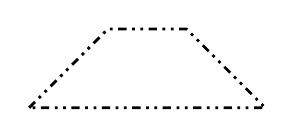
\begin{tikzpicture}
  \coordinate (O) at (0,0);
  \coordinate (A) at (1,1);
  \coordinate (B) at (2,1);
  \coordinate (C) at (3,0);
  \draw[line width = 1, dash dot dot] (O) -- (A) -- (B) --(C) -- cycle;
\end{tikzpicture}
\end{lstlisting}
\normalsize


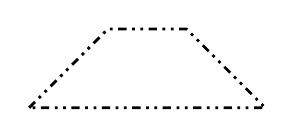
\begin{tikzpicture}
  \coordinate (O) at (0,0);
  \coordinate (A) at (1,1);
  \coordinate (B) at (2,1);
  \coordinate (C) at (3,0);
  \draw[line width = 1, dash dot dot] (O)--(A) -- (B) -- (C) -- cycle;
\end{tikzpicture}

You can draw a rectangle with two points (connecting the diagonal).
For example,



\begin{lstlisting}[language=tex]
\begin{tikzpicture}
  \coordinate (O) at (0,0);
  \coordinate (A) at (1,1);
  \draw[line width = 1, dash dot dot] (O) rectangle (A)
\end{tikzpicture}
\end{lstlisting}



\begin{tikzpicture}
  \coordinate (O) at (0,0);
  \coordinate (A) at (1,1);
  \draw[line width = 1, dash dot dot] (O) rectangle (A);
\end{tikzpicture}

Likewise you can draw a circle with the center and the radius.


\begin{lstlisting}[language=tex]
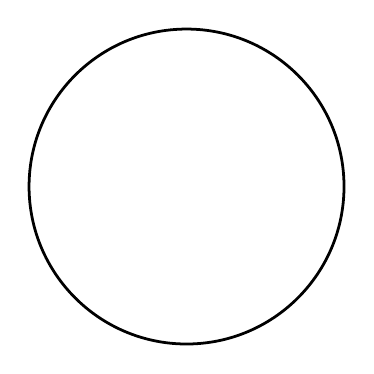
\begin{tikzpicture}
  \coordinate (O) at (0,0);
  \draw[line width = 1]   (O) circle (2);
\end{tikzpicture}
\end{lstlisting}


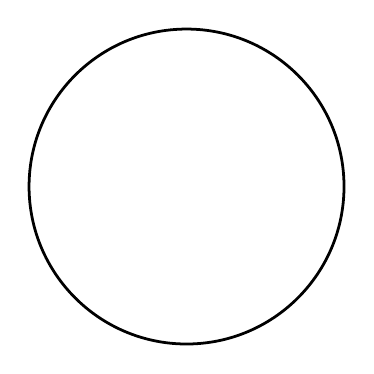
\begin{tikzpicture}
  \coordinate (O) at (0,0);
  \draw[line width = 1]   (O) circle (2);
\end{tikzpicture}

Here we are hard coding the radius $R=2$. We want to use it as a variable.
We show how to do that
\subsection{Defining variables in \myTikZ}
The variables in \myTikZ are defined through the syntax

\begin{alltt}
  \textbackslash{pgfmathsetmacro}\{\textbackslash{variable}\}\{value\} 
\end{alltt}
where the name of the variable is \texttt{\textbackslash variable} and
the value is given by \texttt{value}.

Let us see an example.


\begin{lstlisting}[language=tex]
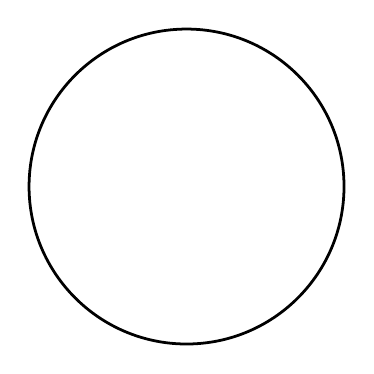
\begin{tikzpicture}
  \pgfmathsetmacro{\R}{2} % units of centimeters
  \coordinate (O) at (0,0);
  \coordinate (A) at (1,1);
  \draw[line width = 1]   (O) circle (\R);
\end{tikzpicture}
\end{lstlisting}

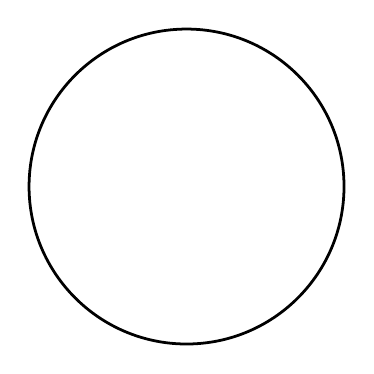
\begin{tikzpicture}
  \pgfmathsetmacro{\R}{2} % units of centimeters
  \coordinate (O) at (0,0);
  \coordinate (A) at (1,1);
  \draw[line width = 1]   (O) circle (\R);
\end{tikzpicture}

We can combine both, the rectangle and the circle as



\begin{lstlisting}[language=tex]
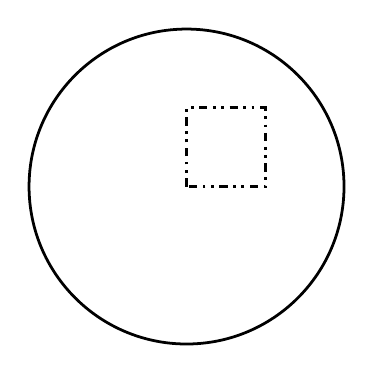
\begin{tikzpicture}
  \pgfmathsetmacro{\R}{2}  % units of points
  \coordinate (O) at (0,0);
  \coordinate (A) at (1,1);
  \draw[line width = 1]   (O) circle (\R);
  \draw[line width = 1, dash dot dot] (O) rectangle (A);
\end{tikzpicture}
\end{lstlisting}

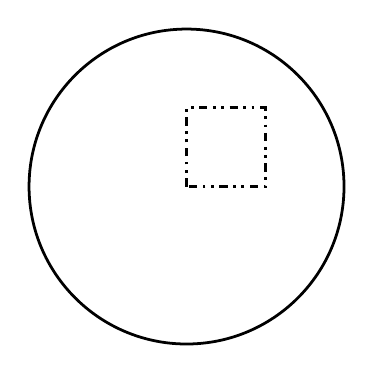
\begin{tikzpicture}
  \pgfmathsetmacro{\R}{2}  % units of points
  \coordinate (O) at (0,0);
  \coordinate (A) at (1,1);
  \draw[line width = 1]   (O) circle (\R);
  \draw[line width = 1, dash dot dot] (O) rectangle (A);
\end{tikzpicture}

\paragraph{Activity \# 1}
There are two options that you can try for \texttt{draw}. These are
\begin{itemize}
  \item opacity and
  \item pattern fills
\end{itemize}
try them on the circle surrounding the rectangle. Opacity actually works well on filled
areas, still try the parameter.

We now try to draw a smooth curve.



\small
\begin{lstlisting}[language=tex]
\begin{tikzpicture}
  \coordinate (O) at (0,0);
  \coordinate (A) at (1,1);
  \coordinate (B) at (2,1);
  \coordinate (C) at (3,0);
  \draw[line width = 1, dash dot dot] (O) -- (A) -- (B) --(C) ;
  \draw[red, thick, smooth] plot coordinates {(O) (A) (B) (C) (D)}; 
\end{tikzpicture}
\end{lstlisting}
\normalsize


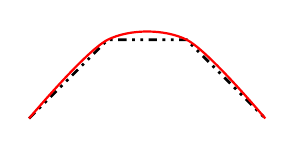
\begin{tikzpicture}
  \coordinate (O) at (0,0);
  \coordinate (A) at (1,1);
  \coordinate (B) at (2,1);
  \coordinate (C) at (3,0);
  \draw[line width = 1, dash dot dot] (O) -- (A) -- (B) --(C) ;
  \draw[red, thick, smooth] plot coordinates {(O) (A) (B) (C) }; % Smooth curve
\end{tikzpicture}

Note that the option \texttt{smooth} requires a different syntax for the  path specification.
The curve is interpolated between the points using  the theory of
\href{https://en.wikipedia.org/wiki/B%C3%A9zier_curve}{B\'ezier curves}.
\footnote{https://en.wikipedia.org/wiki/B\%C3\%A9zier\_curve}

We now show how to draw ellipses.



\begin{lstlisting}[language=tex]
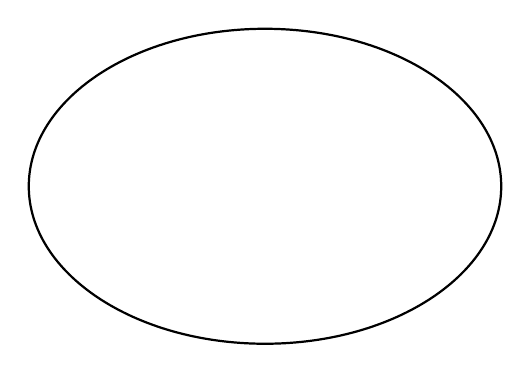
\begin{tikzpicture}
  % Define the ellipse parameters
    \pgfmathsetmacro{\a}{3} % Semi-major axis
    \pgfmathsetmacro{\b}{2} % Semi-minor axis
    
    % Draw the ellipse using calculated parameters
    \draw[black, thick] (0,0) ellipse ({\a} and {\b});
\end{tikzpicture}
\end{lstlisting}


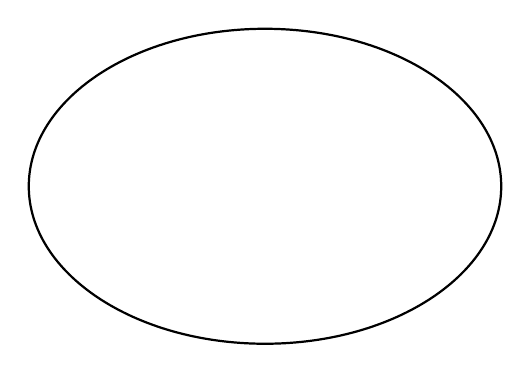
\begin{tikzpicture}
  % Define the ellipse parameters
    \pgfmathsetmacro{\a}{3} % Semi-major axis
    \pgfmathsetmacro{\b}{2} % Semi-minor axis
    
    % Draw the ellipse using calculated parameters
    \draw[black, thick] (0,0) ellipse ({\a} and {\b});
\end{tikzpicture}


\subsection{Arcs in \myTikZ}
Here is a simple arc:

\begin{lstlisting}[language=tex]
\begin{tikzpicture}
    \coordinate (O) at (0,0);
    \pgfmathsetmacro{\startAngle}{0}  % units of degrees
    \pgfmathsetmacro{\endAngle}{90}  % units of degrees
    \pgfmathsetmacro{\R}{2}  % units of points
    % Syntax: \draw[options] (start angle: end angle: radius)
    % Draws a quarter-circle arc
    \draw[blue, thick] (O) arc (\startAngle:\endAngle:\R); 
\end{tikzpicture}
\end{lstlisting}

\begin{tikzpicture}
    \coordinate (O) at (0,0);
    \pgfmathsetmacro{\startAngle}{0}  % units of degrees
    \pgfmathsetmacro{\endAngle}{90}  % units of degrees
    \pgfmathsetmacro{\R}{2}  % units of points
    % Syntax: \draw[options] (start angle: end angle: radius)
    \draw[blue, thick] (O) arc (\startAngle:\endAngle:\R); % Draws a quarter-circle arc
\end{tikzpicture}

We should warn the reader that \texttt{(0)} is not the center of the arc, but the starting
point.

Here is a way to build an arc of parabola using \myTikZ :

\begin{lstlisting}[language=tex]
\begin{tikzpicture}
  \coordinate (O) at (0,0);
  \coordinate (A) at (3,3);
  \draw[] (O) parabola (A);
\end{tikzpicture}
\end{lstlisting}

\begin{tikzpicture}
  \coordinate (O) at (0,0);
  \coordinate (A) at (3,3);
  \draw[] (O) parabola (A);
\end{tikzpicture}

  It is common that we need arrows to indicate some orientation of a curve. 


\subsection{End of curves. Arrows and other}
There is plenty of material about arrows in the 
\href{https://tikz.dev/tikz-arrows}{\myTikZ manual}\footnote{https://tikz.dev/tikz-arrows} .
We only address a few styles here.


\begin{lstlisting}[language=tex]
\begin{tikzpicture}
    \coordinate (O) at (0,0);
    \pgfmathsetmacro{\startAngle}{0}  % units of degrees
    \pgfmathsetmacro{\endAngle}{90}  % units of degrees
    \pgfmathsetmacro{\R}{2}  % units of points
    % Syntax: \draw[options] (start angle: end angle: radius)
    % Draws a quarter-circle arc
    \draw[blue, thick, ->] (O) arc (\startAngle:\endAngle:\R); 
\end{tikzpicture}
\end{lstlisting}

\begin{tikzpicture}
    \coordinate (O) at (0,0);
    \pgfmathsetmacro{\startAngle}{0}  % units of degrees
    \pgfmathsetmacro{\endAngle}{90}  % units of degrees
    \pgfmathsetmacro{\R}{2}  % units of points
    % Syntax: \draw[options] (start angle: end angle: radius)
    \draw[blue, thick, ->] (O) arc (\startAngle:\endAngle:\R); % Draws a quarter-circle arc
\end{tikzpicture}

Note the option \texttt{->}. This is the simplest way to add an arrow at the end of a curve.
There are other options which we will try here.



\begin{lstlisting}[language=tex]
\begin{tikzpicture}
    \coordinate (O) at (0,0);
    \pgfmathsetmacro{\startAngle}{0}  % units of degrees
    \pgfmathsetmacro{\endAngle}{90}  % units of degrees
    \pgfmathsetmacro{\R}{2}  % units of points
    % Syntax: \draw[options] (start angle: end angle: radius)
    \draw[blue, thick, <->] (O) arc (\startAngle:\endAngle:\R); 
\end{tikzpicture}
\end{lstlisting}

\begin{tikzpicture}
    \coordinate (O) at (0,0);
    \pgfmathsetmacro{\startAngle}{0}  % units of degrees
    \pgfmathsetmacro{\endAngle}{90}  % units of degrees
    \pgfmathsetmacro{\R}{2}  % units of points
    % Syntax: \draw[options] (start angle: end angle: radius)
    \draw[blue, thick, <->] (O) arc (\startAngle:\endAngle:\R); 
\end{tikzpicture}

Here \texttt{<->} means double arrow (at the beginning and at the end).


\begin{lstlisting}[language=tex]
\begin{tikzpicture}[scale=2}
    \coordinate (O) at (0,0);
    \pgfmathsetmacro{\startAngle}{0}  % units of degrees
    \pgfmathsetmacro{\endAngle}{90}  % units of degrees
    \pgfmathsetmacro{\R}{2}  % units of points
    % Syntax: \draw[options] (start angle: end angle: radius)
    \draw[blue, thick, -latex] (O) arc (\startAngle:\endAngle:\R); 
\end{tikzpicture}
\end{lstlisting}

\begin{tikzpicture}[scale = 2]
    \coordinate (O) at (0,0);
    \pgfmathsetmacro{\startAngle}{0}  % units of degrees
    \pgfmathsetmacro{\endAngle}{90}  % units of degrees
    \pgfmathsetmacro{\R}{2}  % units of points
    % Syntax: \draw[options] (start angle: end angle: radius)
    \draw[blue, thick, -latex] (O) arc (\startAngle:\endAngle:\R); 
\end{tikzpicture}

Here, another type of arrow. It is called a \texttt{-latex} arrow. Note also that
we used the parameter \texttt{scale=2} at the beginning of the script to make the 
plot larger. We could use also use \texttt{xscale=2} to stretch the figure along the $x$
axis.



\begin{lstlisting}[language=tex]
\begin{tikzpicture}[xscale=2}
    \coordinate (O) at (0,0);
    \pgfmathsetmacro{\startAngle}{0}  % units of degrees
    \pgfmathsetmacro{\endAngle}{90}  % units of degrees
    \pgfmathsetmacro{\R}{2}  % units of points
    % Syntax: \draw[options] (start angle: end angle: radius)
    \draw[blue, thick, -latex] (O) arc (\startAngle:\endAngle:\R); 
\end{tikzpicture}
\end{lstlisting}

\begin{tikzpicture}[xscale = 2]
    \coordinate (O) at (0,0);
    \pgfmathsetmacro{\startAngle}{0}  % units of degrees
    \pgfmathsetmacro{\endAngle}{90}  % units of degrees
    \pgfmathsetmacro{\R}{2}  % units of points
    % Syntax: \draw[options] (start angle: end angle: radius)
    \draw[blue, thick, -latex] (O) 
         arc (\startAngle:\endAngle:\R); % Draws a quarter-circle arc
\end{tikzpicture}

This trick is nice to convert circles into ellipses.

The type of arrows that we have are
\begin{itemize}
  \item \texttt{->} : arrows at the end of the path
  \item \texttt{<-} : arrows at the start of the path
  \item \texttt{<->} : double arrow
  \item \texttt{-stealth} : A stealth shape arrow
\end{itemize}

The arrow tips have also options.
\begin{itemize}
  \item \textbf{type}: the type of arrow is one of the types explained in the previous list. 
    For example, \texttt{-latex}, \texttt{->}, etc.
  \item \textbf{length}: Length of the arrow head
\end{itemize}



\begin{comment}
\begin{lstlisting}[language=tex]
\begin{tikzpicture}[xscale=2}
    \coordinate (O) at (0,0);
    \pgfmathsetmacro{\startAngle}{0}  % units of degrees
    \pgfmathsetmacro{\endAngle}{90}  % units of degrees
    \pgfmathsetmacro{\R}{2}  % units of points
    \draw[-{Latex[length=5mm, width=3mm]}, purple] (O) 
      arc (\startAngle:\endAngle:\R); 
\end{tikzpicture}
\end{lstlisting}
Observe that we can split a line in two (see the instruction \texttt{arc}) with no special 
characters needed.

% for Latex to work you need this line in the preamble
%\usetikzlibrary{arrows.meta}
% after the \usepackage{tikz}
\begin{tikzpicture}[xscale = 2]
    \coordinate (O) at (0,0);
    \pgfmathsetmacro{\startAngle}{0}  % units of degrees
    \pgfmathsetmacro{\endAngle}{90}  % units of degrees
    \pgfmathsetmacro{\R}{2}  % units of points
    % Syntax: \draw[options] (start angle: end angle: radius)
    \draw[-{Latex[length=5mm, width=3mm]}, purple] (O) arc (\startAngle:\endAngle:\R); 
\end{tikzpicture}
\end{comment}

To use the \texttt{Latex} directive above we need to include the \texttt{arrows.meta} library.

Tha is, 

\begin{lstlisting}[language=tex]
  \usetikzlibrary{arrows.meta}
\end{lstlisting}

Note that we change the length and witdth of the arrow. We changed also the color
of the curve. There are plenty of more options in the
\href{https://tikz.dev/tikz-arrows}{\myTikZ manual}
\footnote{https://tikz.dev/tikz-arrows} 
which we will not consider here. We suggest to the student to visit the manual for more
on arrows and ending shapes of curves.

\paragraph{Activity \# 2}: Make a curve with an arrow at the end. The color of the
curve is black and that of the arrow is blue.
\vspace{0.5in}


\subsubsection{Make a grid}
The key line here is:
\begin{lstlisting}[language=tex]
    \draw[ step=1cm, gray, very thin] (G) grid (A);
\end{lstlisting}

We draw a grid around the arc defined above.


\begin{lstlisting}[language=tex]
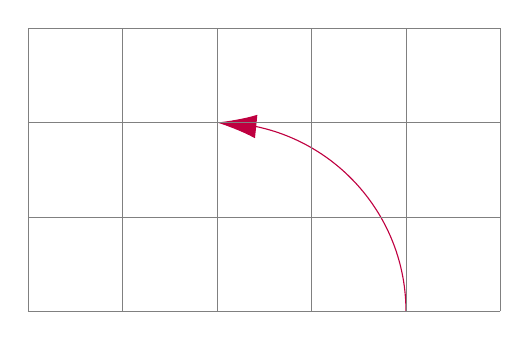
\begin{tikzpicture}[scale = 1.2]
    \pgfmathsetmacro{\startAngle}{0}  % units of degrees
    \pgfmathsetmacro{\endAngle}{90}  % units of degrees
    \pgfmathsetmacro{\R}{2}  % units of points
    % Syntax: \draw[options] (start angle: end angle: radius)
    \coordinate (O) at (0,0);
    \coordinate (A) at (2,0);
    \draw[-{Latex[length=5mm, width=3mm]}, purple] (A) 
       arc (\startAngle:\endAngle:\R); 
    \coordinate (G) at (-2,0);
    \coordinate (A) at (3,3);
    \draw[ step=1cm, gray, very thin] (G) grid (A);
\end{tikzpicture}
\end{lstlisting}


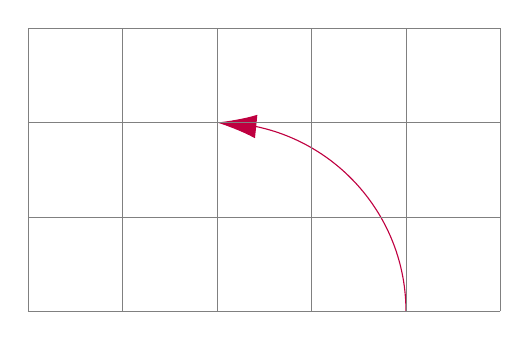
\begin{tikzpicture}[scale = 1.2]
    \pgfmathsetmacro{\startAngle}{0}  % units of degrees
    \pgfmathsetmacro{\endAngle}{90}  % units of degrees
    \pgfmathsetmacro{\R}{2}  % units of points
    % Syntax: \draw[options] (start angle: end angle: radius)
    \coordinate (O) at (0,0);
    \coordinate (A) at (2,0);
    \draw[-{Latex[length=5mm, width=3mm]}, purple] (A) 
       arc (\startAngle:\endAngle:\R); 
    \coordinate (G) at (-2,0);
    \coordinate (A) at (3,3);
    \draw[ step=1cm, gray, very thin] (G) grid (A);
\end{tikzpicture}

\subsection{The fill and shade}

\begin{lstlisting}[language=tex]
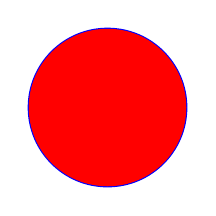
\begin{tikzpicture}
  \pgfmathsetmacro{\R}{1}  % units of points
  \coordinate (O) at (0,0);
  \draw[thick, blue] (0,0) circle (1); % Outline of the circle
   % Filling a circle with a color
  \fill[red] (O) circle (\R); % Fill the circle with red color
\end{tikzpicture}
\end{lstlisting}

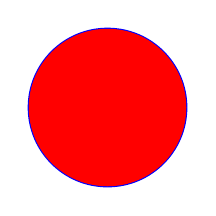
\begin{tikzpicture}
  \pgfmathsetmacro{\R}{1}  % units of points
  \coordinate (O) at (0,0);
  \draw[thick, blue] (O) circle (1); % Outline of the circle
   % Filling a circle with a color
  \fill[red] (O) circle (\R); % Fill the circle with red color
\end{tikzpicture}

You can do both tasks (draw the border and fill) at the same time with the
instruction \texttt{\textbackslash filldraw}. Let us see


\begin{lstlisting}[language=tex]
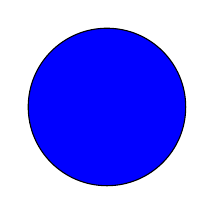
\begin{tikzpicture}
  \pgfmathsetmacro{\R}{1}  % units of points
  \coordinate (O) at (0,0);
   % Filling a circle with a color and draw boundary
  \filldraw[fill=blue, draw=black] (O) circle (\R); 
\end{tikzpicture}
\end{lstlisting}

\begin{tikzpicture}
  \pgfmathsetmacro{\R}{1}  % units of points
  \coordinate (O) at (0,0);
   % Filling a circle with a color and draw boundary
  \filldraw[fill=blue, draw=black] (O) circle (\R); 
\end{tikzpicture}



\begin{lstlisting}[language=tex]
\begin{tikzpicture}
  \pgfmathsetmacro{\R}{1}  % units of points
  \coordinate (O) at (0,0);
   % shading a circle
  \shade[left color=blue, right color=red] (O) circle (\R); 
\end{tikzpicture}
\end{lstlisting}

\begin{tikzpicture}
  \pgfmathsetmacro{\R}{1}  % units of points
  \coordinate (O) at (0,0);
   % shading a circle
  \shade[left color=blue, right color=red] (O) circle (\R); 
  %\shade[inner color=blue, outer color=red] (O) circle (\R); 
  %\shade[top color=blue, bottom color=red] (O) circle (\R); 
  %\shade[bottom color=blue, top color=red] (O) circle (\R); 
\end{tikzpicture}

Shade works also from top to bottom, bottom to top, inner to out, or out to inner. 
We leave this kind of shade to the student

\paragraph{Activity \# 3}
Shade the circle above from top to bottom,  bottom to top, inner to outer, and 
outer to inner.

\subsection{Axes}
Axes are easily included. Let us copy the script with the arc in a grid and
add the axes to it, after a few modifications; mainly the scaling and the
starting of the arc, for a more pleasant  display.



\begin{lstlisting}[language=tex]
\begin{tikzpicture}[scale = 1.2]
    \pgfmathsetmacro{\startAngle}{0}  % units of degrees
    \pgfmathsetmacro{\endAngle}{90}  % units of degrees
    \pgfmathsetmacro{\R}{2}  % units of points
    % Syntax: \draw[options] (start angle: end angle: radius)
    \coordinate (O) at (0,0);
    \coordinate (A) at (2,0);
    \draw[-{Latex[length=5mm, width=3mm]}, purple] (A) 
       arc (\startAngle:\endAngle:\R); 
    \coordinate (G) at (-2,0);
    \coordinate (A) at (3,3);
    \draw[ step=1cm, gray, very thin] (G) grid (A);

    \coordinate (OX) at (2,0);
    \coordinate (Oy) at (0,2);

    \draw[line width=2, -latex] (O) -- (OX);
    \draw[line width=2, -latex] (O) -- (Oy);
\end{tikzpicture}
\end{lstlisting}


\begin{tikzpicture}[scale = 1.2]
    \pgfmathsetmacro{\startAngle}{0}  % units of degrees
    \pgfmathsetmacro{\endAngle}{90}  % units of degrees
    \pgfmathsetmacro{\R}{2}  % units of points
    % Syntax: \draw[options] (start angle: end angle: radius)
    \coordinate (O) at (0,0);
    \coordinate (A) at (2,0);
    \draw[-{Latex[length=5mm, width=3mm]}, purple] (A) 
       arc (\startAngle:\endAngle:\R); 
    \coordinate (G) at (-2,0);
    \coordinate (A) at (3,3);
    \draw[ step=1cm, gray, very thin] (G) grid (A);

    \coordinate (OX) at (2,0);
    \coordinate (Oy) at (0,2);

    \draw[line width=2, -latex] (O) -- (OX);
    \draw[line width=2, -latex] (O) -- (Oy);
\end{tikzpicture}


At this point we are in need to put some labels. We introduce the
\texttt{node} directive.

\subsection{The \texttt{node} and \texttt{\textbackslash node} directives}

There are two ways to use the string \texttt{node} in \myTikZ,  one with
no \texttt{\textbackslash} and the other with \texttt{\textbackslash}.
The \texttt{node} with no backslash is used directly in the line that starts with 
\texttt{\textbackslash draw}. Here is an example with no backslash.

\begin{lstlisting}[language=tex]
\begin{tikzpicture}[scale = 1.2]
    \pgfmathsetmacro{\startAngle}{0}  % units of degrees
    \pgfmathsetmacro{\endAngle}{90}  % units of degrees
    \pgfmathsetmacro{\R}{2}  % units of points
    % Syntax: \draw[options] (start angle: end angle: radius)
    \coordinate (O) at (0,0);
    \coordinate (A) at (2,0);
    \draw[-{Latex[length=5mm, width=3mm]}, purple] (A) 
       arc (\startAngle:\endAngle:\R); 
    \coordinate (G) at (-2,0);
    \coordinate (A) at (3,3);
    \draw[ step=1cm, gray, very thin] (G) grid (A);

    \coordinate (OX) at (2,0);
    \coordinate (Oy) at (0,2);

    \draw[line width=2, -latex] (O) -- (OX) node[right] {$x$ axis};
    \draw[line width=2, -latex] (O) -- (Oy) node[above] {$y$ axis};
\end{tikzpicture}
\end{lstlisting}


\begin{tikzpicture}[scale = 1.2]
    \pgfmathsetmacro{\startAngle}{0}  % units of degrees
    \pgfmathsetmacro{\endAngle}{90}  % units of degrees
    \pgfmathsetmacro{\R}{2}  % units of points
    % Syntax: \draw[options] (start angle: end angle: radius)
    \coordinate (O) at (0,0);
    \coordinate (A) at (2,0);
    \draw[-{Latex[length=5mm, width=3mm]}, purple] (A) 
       arc (\startAngle:\endAngle:\R); 
    \coordinate (G) at (-2,0);
    \coordinate (A) at (3,3);
    \draw[ step=1cm, gray, very thin] (G) grid (A);

    \coordinate (OX) at (2,0);
    \coordinate (Oy) at (0,2);

    \draw[line width=2, -latex] (O) -- (OX) node[right] {$x$ axis};
    \draw[line width=2, -latex] (O) -- (Oy) node[above] {$y$ axis};
\end{tikzpicture}

We now illustrate the use of  \texttt{\textbackslash node} ,
%\texttt{textbackslash node}.


\begin{lstlisting}[language=tex]
\begin{tikzpicture}[scale = 1.2]
    \pgfmathsetmacro{\startAngle}{0}  % units of degrees
    \pgfmathsetmacro{\endAngle}{90}  % units of degrees
    \pgfmathsetmacro{\R}{2}  % units of points
    % Syntax: \draw[options] (start angle: end angle: radius)
    \coordinate (O) at (0,0);
    \coordinate (A) at (2,0);
    \draw[-{Latex[length=5mm, width=3mm]}, purple] (A) 
       arc (\startAngle:\endAngle:\R); 
    \coordinate (G) at (-2,0);
    \coordinate (A) at (3,3);
    \draw[ step=1cm, gray, very thin] (G) grid (A);

    \coordinate (OX) at (3,0);
    \coordinate (Oy) at (0,3);

    \draw[line width=2, -latex] (O) -- (OX) node[right] {$x$};
    \draw[line width=2, -latex] (O) -- (Oy) node[above] {$y$};


    \coordinate (M) at (2,2);
    \node[above] at (M) {This is an arc };
\end{tikzpicture}
\end{lstlisting}



\begin{tikzpicture}[scale = 1.2]
    \pgfmathsetmacro{\startAngle}{0}  % units of degrees
    \pgfmathsetmacro{\endAngle}{90}  % units of degrees
    \pgfmathsetmacro{\R}{2}  % units of points
    % Syntax: \draw[options] (start angle: end angle: radius)
    \coordinate (O) at (0,0);
    \coordinate (A) at (2,0);
    \draw[-{Latex[length=5mm, width=3mm]}, purple] (A) 
       arc (\startAngle:\endAngle:\R); 
    \coordinate (G) at (-2,0);
    \coordinate (A) at (3,3);
    \draw[ step=1cm, gray, very thin] (G) grid (A);

    \coordinate (OX) at (3,0);
    \coordinate (Oy) at (0,3);

    \draw[line width=2, -latex] (O) -- (OX) node[right] {$x$};
    \draw[line width=2, -latex] (O) -- (Oy) node[above] {$y$};

    \coordinate (M) at (2,2);
    \node[above] at (M) {This is an arc };


\end{tikzpicture}



There are many options for \texttt{node} (with or without backslash), some of them are:
\begin{itemize}
  \item scale: scales the node.
  \item rotate: rotate the node.
  \item below: locates the node below the reference coordinate (in the example above the
      coordinate is $(2,2)$.
    \item above: locates the node output above the coordinate.
    \item left: locates the node output to the left of the coordinate.
    \item right : locates the node output to the right of the coordinate.
  \item below right: locates the node output below to the right of the coordinate.
  \item below left: locates the node output below and to the left of the coordinate.
  \item above  right locates the node output above and to the right of the coordinate.
  \item above  left: locates the node output above and to the left of the coordinate.
  \item xshift: This good for fine tunning the location of your node. Usually small quantities
    shift the node to the right or to the left. For example $-2mm$ to the left and $2mm$ to the
    right.
  \item yshift: This, like the previous, shifts the node up or down.
\end{itemize}

\paragraph{Activity \#  4}
Try all the options on \texttt{\textbackslash node} above.

It is interesting that there is not a \texttt{print} statement in \myTikZ. However
the \texttt{node} directive serves as a print for any variable in the program or any 
message that want to be display with the graphic. In this way the \texttt{node} 
(with or without backslash) helps on debugging \myTikZ code.

\section{Control flow instructions: loops and if statements}
\subsection{The \texttt{\textbackslash foreach} loop}
We will put ticks on the figure with grid and axis.

\small
\begin{lstlisting}[language=tex]
\begin{tikzpicture}[scale = 1.2]
    \pgfmathsetmacro{\startAngle}{0}  % units of degrees
    \pgfmathsetmacro{\endAngle}{90}  % units of degrees
    \pgfmathsetmacro{\R}{2}  % units of points
    % Syntax: \draw[options] (start angle: end angle: radius)
    \coordinate (O) at (0,0);
    \coordinate (A) at (2,0);
    \draw[-{Latex[length=5mm, width=3mm]}, purple] (A) 
       arc (\startAngle:\endAngle:\R); 
    \coordinate (G) at (-2,0);
    \coordinate (A) at (3,3);
    \draw[ step=1cm, gray, very thin] (G) grid (A);

    \coordinate (OX) at (3,0);
    \coordinate (Oy) at (0,3);

    \draw[line width=2, -latex] (O) -- (OX) node[right] {$x$};
    \draw[line width=2, -latex] (O) -- (Oy) node[above] {$y$};

    \foreach \x in {0,1,2,3}
        \draw (\x cm,1pt) -- (\x cm,-1pt) node[anchor=north]{$\x$};
    \foreach \y in {0,1,2,3}
        \draw (1pt,\y cm) -- (-1pt,\y cm) node[anchor=east]{$\y$};

    \coordinate (M) at (2,2);
    \node[above] at (M) {This is an arc };
\end{tikzpicture}
\end{lstlisting}
\normalsize



\begin{tikzpicture}[scale = 1.2]
    \pgfmathsetmacro{\startAngle}{0}  % units of degrees
    \pgfmathsetmacro{\endAngle}{90}  % units of degrees
    \pgfmathsetmacro{\R}{2}  % units of points
    % Syntax: \draw[options] (start angle: end angle: radius)
    \coordinate (O) at (0,0);
    \coordinate (A) at (2,0);
    \draw[-{Latex[length=5mm, width=3mm]}, purple] (A) 
       arc (\startAngle:\endAngle:\R); 
    \coordinate (G) at (-2,0);
    \coordinate (A) at (3,3);
    \draw[ step=1cm, gray, very thin] (G) grid (A);

    \coordinate (OX) at (3,0);
    \coordinate (Oy) at (0,3);

    \draw[line width=2, -latex] (O) -- (OX) node[right] {$x$};
    \draw[line width=2, -latex] (O) -- (Oy) node[above] {$y$};

    \foreach \x in {0,1,2,3}
        \draw (\x cm,1pt) -- (\x cm,-1pt) node[anchor=north]{$\x$};
    \foreach \y in {0,1,2,3}
        \draw (1pt,\y cm) -- (-1pt,\y cm) node[anchor=east]{$\y$};

    \coordinate (M) at (2,2);
    \node[above] at (M) {This is an arc };
\end{tikzpicture}

The \texttt{\textbackslash foreach} loop can be extended for more general ranges.
In the following example we show that a few first values will define the increment and
you can fix the last position. We make the grid double as fine on each direction.


\begin{lstlisting}[language=tex]
\begin{tikzpicture}[scale = 1.2]
    \pgfmathsetmacro{\startAngle}{0}  % units of degrees
    \pgfmathsetmacro{\endAngle}{90}  % units of degrees
    \pgfmathsetmacro{\R}{2}  % units of points
    % Syntax: \draw[options] (start angle: end angle: radius)
    \coordinate (O) at (0,0);
    \coordinate (A) at (2,0);
    \draw[-{Latex[length=5mm, width=3mm]}, purple] (A) 
       arc (\startAngle:\endAngle:\R); 
    \coordinate (G) at (-2,0);
    \coordinate (A) at (3,3);
    \draw[ step=0.5cm, gray, very thin] (G) grid (A);

    \coordinate (OX) at (3,0);
    \coordinate (Oy) at (0,3);

    \draw[line width=2, -latex] (O) -- (OX) node[right] {$x$};
    \draw[line width=2, -latex] (O) -- (Oy) node[above] {$y$};

    \foreach \x in {0, 0.5, 1, 1.5, ..., 3} 
        \draw (\x cm,1pt) -- (\x cm,-1pt) node[anchor=north] {$\x$};
    \foreach \y in {0, 0.5, 1, 1.5, ..., 3} 
        \draw (1pt,\y cm) -- (-1pt,\y cm) node[anchor=east] {$\y$};

    \coordinate (M) at (2,2);
    \node[above] at (M) {This is an arc };
\end{tikzpicture}
\end{lstlisting}


\begin{tikzpicture}[scale = 1.2]
    \pgfmathsetmacro{\startAngle}{0}  % units of degrees
    \pgfmathsetmacro{\endAngle}{90}  % units of degrees
    \pgfmathsetmacro{\R}{2}  % units of points
    % Syntax: \draw[options] (start angle: end angle: radius)
    \coordinate (O) at (0,0);
    \coordinate (A) at (2,0);
    \draw[-{Latex[length=5mm, width=3mm]}, purple] (A) 
       arc (\startAngle:\endAngle:\R); 
    \coordinate (G) at (-2,0);
    \coordinate (A) at (3,3);
    \draw[ step=0.5cm, gray, very thin] (G) grid (A);

    \coordinate (OX) at (3,0);
    \coordinate (Oy) at (0,3);

    \draw[line width=2, -latex] (O) -- (OX) node[right] {$x$};
    \draw[line width=2, -latex] (O) -- (Oy) node[above] {$y$};

    \foreach \x in {0, 0.5, 1, 1.5, ..., 3} 
        \draw (\x cm,1pt) -- (\x cm,-1pt) node[anchor=north] {$\x$};
    \foreach \y in {0, 0.5, 1, 1.5, ..., 3} 
        \draw (1pt,\y cm) -- (-1pt,\y cm) node[anchor=east] {$\y$};

    \coordinate (M) at (2,2);
    \node[above] at (M) {This is an arc };
\end{tikzpicture}


\vspace{1in}
Finally, we will show an example of how to construct a neural network to explain the
matrix vector product. There are packages already built to draw Neural networks, we show
them at the end of this notes.

\small
\begin{lstlisting}[language=tex]
\begin{center}
  \begin{tikzpicture}

    \foreach \t in {0,1,...,5} {
      \draw[] (0, \t) circle(4pt);
    }

    \foreach \t in {-2, 0, ..., 6} {
      \draw[] (5, \t) circle(4pt);
    }

      % node k in the arriving layer
    \coordinate (B2) at (5, 0);
    \node[right] at (B2) {\Large $z_k$};
    \coordinate (B3) at (5, 6);
    \node[right] at (B3) {\Large $z_1$};
    \coordinate (B4) at (5, -2);
    \node[right] at (B4) {\Large $z_n$};
    \fill[green] (B2) circle (4pt);

    \foreach \x in {0,1,...,5} {
      \foreach \y in {-2,0,...,6} {
        \draw[] (0, \x) -- (5, \y);
      }
    }

    \draw[line width=2, color=red] (0,3)--(B2);
    \coordinate (theta) at (2.5, 1.5);
    \node[above] at (theta) {\large $\textcolor{red}{\bf \theta_{ki}}$};
    \node[left] at (-0.2,3) {\large $x_i$};
    \node[left] at (-0.2,0) {\large $x_m$};
    \node[left] at (-0.2,5) {\large $x_1$};

    \coordinate (A) at (0,5.2);
    \coordinate (B) at (5,6.2);
    \node[above] at (A) {A};
    \node[above] at (B) {B};

  \end{tikzpicture}
\end{center}
\end{lstlisting}
\normalsize

\begin{center}
  \begin{tikzpicture}

    \foreach \t in {0,1,...,5} {
      \draw[] (0, \t) circle(4pt);
    }

    \foreach \t in {-2, 0, ..., 6} {
      \draw[] (5, \t) circle(4pt);
    }

      % node k in the arriving layer
    \coordinate (B2) at (5, 0);
    \node[right] at (B2) {\Large $z_k$};
    \coordinate (B3) at (5, 6);
    \node[right] at (B3) {\Large $z_1$};
    \coordinate (B4) at (5, -2);
    \node[right] at (B4) {\Large $z_n$};
    \fill[green] (B2) circle (4pt);

    \foreach \x in {0,1,...,5} {
      \foreach \y in {-2,0,...,6} {
        \draw[] (0, \x) -- (5, \y);
      }
    }

    \draw[line width=2, color=red] (0,3)--(B2);
    \coordinate (theta) at (2.5, 1.5);
    \node[above] at (theta) {\large $\textcolor{red}{\theta_{ki}}$};
    \node[left] at (-0.2,3) {\large $x_i$};
    \node[left] at (-0.2,0) {\large $x_m$};
    \node[left] at (-0.2,5) {\large $x_1$};

    \coordinate (A) at (0,5.2);
    \coordinate (B) at (5,6.2);
    \node[above] at (A) {A};
    \node[above] at (B) {B};

  \end{tikzpicture}
\end{center}



\subsection{The \texttt{\textbackslash if} statement}
The following example, generated by ChatGPT, shows the use of the \texttt{if} statement in
\myTikZ.  The instruction \\ \texttt{\textbackslash def\textbackslash myvalue} \\ is a macro
from \myLaTeX . It does not belong to \myTikZ.

\begin{lstlisting}[language=tex]
\begin{tikzpicture}
    % Define a variable
    \def\myvalue{5}
    
    % Conditional statement to draw different shapes
    \ifnum\myvalue<5
        \draw[red] (0,0) circle (1);
    \else
        \draw[blue] (0,0) rectangle (2,2);
    \fi
\end{tikzpicture}
\end{lstlisting}


\begin{tikzpicture}
    % Define a variable
    \def\myvalue{5}
    
    % Conditional statement to draw different shapes
    \ifnum\myvalue<5
        \draw[red] (0,0) circle (1);
    \else
        \draw[blue] (0,0) rectangle (2,2);
    \fi
\end{tikzpicture}

The script decides if drawing a circle (if the number \texttt{\textbackslash myvalue} is
smaller than 5), or a rectangle (if the number \texttt{\textbackslash myvalue} is smaller or
equal than 5). Since the number is equal to $5$ a rectangle is drawn.


\section{Mathematics in \myTikZ}
\myTikZ is not a package to do math. However some complex programs could need some
mathematical computations. We show how do do math operations with \myTikZ. 

Here is a script with some simple math.

\begin{lstlisting}[language=tex]
\begin{tikzpicture}
    % Define variables
    \pgfmathsetmacro{\a}{3}
    \pgfmathsetmacro{\b}{7}
    
    % Perform arithmetic operations
    \pgfmathsetmacro{\sum}{\a + \b}
    \pgfmathsetmacro{\difference}{\b - \a}
    \pgfmathsetmacro{\product}{\a * \b}
    \pgfmathsetmacro{\quotient}{\b / \a}
    
    % Display results
    \node at (0,0) {Sum: $\sum$};
    \node at (0,-0.5) {Difference: $\difference$};
    \node at (0,-1) {Product: $\product$};
    \node at (0,-1.5) {Quotient: $\quotient$};
\end{tikzpicture}

\end{lstlisting}

\begin{tikzpicture}
    % Define variables
    \pgfmathsetmacro{\a}{3}
    \pgfmathsetmacro{\b}{7}
    
    % Perform arithmetic operations
    \pgfmathsetmacro{\sum}{\a + \b}
    \pgfmathsetmacro{\difference}{\b - \a}
    \pgfmathsetmacro{\product}{\a * \b}
    \pgfmathsetmacro{\quotient}{\b / \a}
    
    % Display results
    \node at (0,0) {Sum: $\sum$};
    \node at (0,-0.5) {Difference: $\difference$};
    \node at (0,-1) {Product: $\product$};
    \node at (0,-1.5) {Quotient: $\quotient$};
\end{tikzpicture}

The idea is not to do complicated math but use some math for complex graphics that
require it.

We can do more complex math such as trigonometrical, logarithm, and exponential functions.

\begin{lstlisting}[language=tex]
\begin{tikzpicture}
    % Trigonometric functions
    \pgfmathsetmacro{\angle}{30}
    \pgfmathsetmacro{\sine}{sin(\angle)}
    \pgfmathsetmacro{\cosine}{cos(\angle)}
    \pgfmathsetmacro{\tangent}{tan(\angle)}
    
    % Exponential and logarithmic functions
    \pgfmathsetmacro{\exponential}{exp(1)}
    \pgfmathsetmacro{\lnValue}{ln(5)}
    
    % Display results
    \node at (0,3) {Trigonometric Functions:};
    \node at (0,2.5) {$\sin(\angle) = \sine$};
    \node at (0,2) {$\cos(\angle) = \cosine$};
    \node at (0,1.5) {$\tan(\angle) = \tangent$};
    
    \node at (0,0.5) {Exponential and Logarithmic Functions:};
    \node at (0,0) {$e = \exponential$};
    \node at (0,-0.5) {$\ln(5) = \lnValue$};
\end{tikzpicture}
\end{lstlisting}


\begin{tikzpicture}
    % Trigonometric functions
    \pgfmathsetmacro{\angle}{30}
    \pgfmathsetmacro{\sine}{sin(\angle)}
    \pgfmathsetmacro{\cosine}{cos(\angle)}
    \pgfmathsetmacro{\tangent}{tan(\angle)}
    
    % Exponential and logarithmic functions
    \pgfmathsetmacro{\exponential}{exp(1)}
    \pgfmathsetmacro{\lnValue}{ln(5)}
    
    % Display results
    \node at (0,3) {Trigonometric Functions:};
    \node at (0,2.5) {$\sin(\angle) = \sine$};
    \node at (0,2) {$\cos(\angle) = \cosine$};
    \node at (0,1.5) {$\tan(\angle) = \tangent$};
    
    \node at (0,0.5) {Exponential and Logarithmic Functions:};
    \node at (0,0) {$e = \exponential$};
    \node at (0,-0.5) {$\ln(5) = \lnValue$};
\end{tikzpicture}

\paragraph{Activity \# 5:}
Write a \myTikZ script that draws a right triangle with vertices $(0,0), (4,0), (0,3)$.
Compute, using the Pythagoras theorem, the length of the hypotenuse and write this
in a text above the hypotenuse tilted so that it is parallel to it.
Write also the angle at the vertex  $(4,0)$. In other words, write a script that
shows the following figure.


\begin{tikzpicture}
    % Define triangle vertices
    \coordinate (A) at (0,0);
    \coordinate (B) at (0,3);
    \coordinate (C) at (4,0);
    
    % Draw triangle
    \draw (A) -- (B) -- (C) -- cycle;
    
    % Compute the length of the hypotenuse
    \pgfmathsetmacro{\sideA}{3}
    \pgfmathsetmacro{\sideB}{4}
    \pgfmathsetmacro{\hypotenuse}{sqrt(\sideA^2 + \sideB^2)}
    
    % Label sides of the triangle
    \node[below left] at (A) {$(0,0)$};
    \node[left] at (B) {$(0,3)$};
    \node[below right] at (C) {$(4,0)$};
    
    % compute the angle for the text
    \pgfmathsetmacro{\angle}{atan(\sideA/\sideB)}



    % Label the hypotenuse length
    %\node[above, sloped] at ($(B)!.5!(C)$) {\small Hypotenuse: $\hypotenuse$};
    \node[above right, rotate=-\angle] at (B) {\small Hypotenuse: $\hypotenuse$};
    \node[above left, xshift=-1cm] at (C) {\small Angle: $\angle$};



    \pgfmathsetmacro{\startAngle}{180}  % units of degrees
    \pgfmathsetmacro{\endAngle}{180-\angle}
    \pgfmathsetmacro{\R}{1.0}  % units of points
    \coordinate (A) at (3,0);
     \draw[->, purple] (A) 
       arc (\startAngle:\endAngle:\R); 

    \node [above, yshift=-2pt] at (3.3,0) {$\theta$};

    % \node[] at (5,0) {end angle = \endAngle};
\end{tikzpicture}

Please observe the arc at the vertix $(4,0)$. The starting angle is $180$, find the
ending angle based on the acute angle at the vertix. Compute the ending angle using
\texttt{{\textbackslash}pgfmathsetmacro}. You will need to figure out what radius $R$ is good to 
get the figure right. A small radius $R$, such as $R=0.2$ will not extend the arc all the
way to hit the side. Recall that arc $S$ is equal to $S=R \theta$, where $\theta$ is the angle.




\section{Graphing functions}
Graphing functions is easy with \myTikZ.  Here is a script to graph the function $y = \sin x$.

\begin{lstlisting}[language=tex]
\begin{tikzpicture}[scale=1.5]
    % Axes
    \draw[->] (-2,0) -- (2,0) node[right] {$x$};
    \draw[->] (0,-1.5) -- (0,1.5) node[above] {$y$};
    
    % Sine function
    \draw[domain=-1.8:1.8,smooth,variable=\x,blue] 
        plot (\x,{sin(180*\x)});
    
    % Equation labels
    \node[below right,blue] at (1.5,1) {$y = \sin(x)$};
    
\end{tikzpicture}
\end{lstlisting}



\begin{tikzpicture}[scale=1.5]
    % Axes
    \draw[->] (-2,0) -- (2,0) node[right] {$x$};
    \draw[->] (0,-1.5) -- (0,1.5) node[above] {$y$};
    
    % Sine function
    \draw[domain=-1.8:1.8,smooth,variable=\x,blue] plot (\x,{sin(180*\x)});
    
    % Equation labels
    \node[below right,blue] at (1.5,1) {$y = \sin(x)$};
    
\end{tikzpicture}

Note that we hard-coded the coordinates and other numerical parameters to make the 
script short. However when writing professional code this should not be done.

\subsection{Plots using \texttt{\textbackslash addplot} and \texttt{axis}}
There is an environment

\begin{lstlisting}[language=tex]
  \begin{axis}
    do things here
  \end{axis}
\end{lstlisting}
which is quite useful for plotting functions. Here is an example of how
this works. It is flexible to include several 2D graphs.


\small
\begin{lstlisting}[language=tex]
\begin{tikzpicture}
    \begin{axis}[
        axis lines=middle,
        xlabel=$x$,
        ylabel=$y$,
        xmin=-2, xmax=2,
        ymin=-1, ymax=3,
        grid=both,
        width=10cm,
        height=7cm,
        samples=100 % Number of samples for smooth curve
    ]
    
    % Plot the function
     % Function: y = x^2
    \addplot[blue, domain=-2:2, line width=2] {x^2} 
        node[pos=0.8, below right, xshift=-10pt] {$y=x^2$}; 
    % Mark some key points
    \node[label={180:{$(0,0)$}},circle,fill,inner sep=2pt] 
         at (axis cs:0,0) {};
    \node[label={180:{$(1,1)$}},circle,fill,inner sep=2pt] 
         at (axis cs:1,1) {};
    

    
    % Function: y=3 sin(x*180/pi)
    \addplot[red, line width=2,  domain=-2:2] {3*sin(x*180/pi)}; 
    % Function: y=1-exp(-x)
    \addplot[green, line width=2, domain=-2:2] {1-exp(-x))}; 
    
    \end{axis}
\end{tikzpicture}
\end{lstlisting}
\normalsize

\begin{tikzpicture}
    \begin{axis}[
        axis lines=middle,
        xlabel=$x$,
        ylabel=$y$,
        xmin=-2, xmax=2,
        ymin=-1, ymax=3,
        grid=both,
        width=10cm,
        height=7cm,
        samples=100 % Number of samples for smooth curve
    ]
    
    % Plot the function
     % Function: y = x^2
    \addplot[blue, domain=-2:2, line width=2] {x^2} 
        node[pos=0.8, below right, xshift=-10pt] {$y=x^2$}; 
    % Mark some key points
      \node[label={180:{$(0,0)$}}, circle, fill, inner sep=2pt] at (axis cs:0,0) {};
       \node[label={180:{$(1,1)$}},
        circle,fill,inner sep=2pt] at (axis cs:1,1) {};
    

    
    % Function: y=3 sin(x*180/pi)
    \addplot[red, line width=2,  domain=-2:2] {3*sin(x*180/pi)}; 
    % Function: y=1-exp(-x)
    \addplot[green, line width=2, domain=-2:2] {1-exp(-x))}; 
    
    \end{axis}
\end{tikzpicture}

\paragraph{Activity \# 6:}
Add labels, on the previous figure, for the sinusoidal function and the exponential function.

\section{Three dimensional graphs}
The following example, generated with ChatGPT shows a figure using 3D coordinates.

\begin{lstlisting}[language=tex]
\begin{tikzpicture}[scale=1.5]

  % Define coordinates
  \coordinate (A) at (0,0,0);
  \coordinate (B) at (1,0,0);
  \coordinate (C) at (1,1,0);
  \coordinate (D) at (0,1,0);
  \coordinate (E) at (0,0,1);
  \coordinate (F) at (1,0,1);
  \coordinate (G) at (1,1,1);
  \coordinate (H) at (0,1,1);

% Draw the edges of the cube
  \draw (A) -- (B) -- (C) -- (D) -- cycle;
  \draw (E) -- (F) -- (G) -- (H) -- cycle;
  \draw (A) -- (E);
  \draw (B) -- (F);
  \draw (C) -- (G);
  \draw (D) -- (H);

% Show vertices
  \foreach \vertex in {A,B,C,D,E,F,G,H}
      \fill [black] (\vertex) circle (1.5pt) node {\vertex};
      

\end{tikzpicture}
\end{lstlisting}

\begin{tikzpicture}[scale=1.5]

  % Define coordinates
  \coordinate (A) at (0,0,0);
  \coordinate (B) at (1,0,0);
  \coordinate (C) at (1,1,0);
  \coordinate (D) at (0,1,0);
  \coordinate (E) at (0,0,1);
  \coordinate (F) at (1,0,1);
  \coordinate (G) at (1,1,1);
  \coordinate (H) at (0,1,1);

% Draw the edges of the cube
  \draw (A) -- (B) -- (C) -- (D) -- cycle;
  \draw (E) -- (F) -- (G) -- (H) -- cycle;
  \draw (A) -- (E);
  \draw (B) -- (F);
  \draw (C) -- (G);
  \draw (D) -- (H);

% Show vertices
  \foreach \vertex in {A,B,C,D,E,F,G,H}
      \fill [black] (\vertex) circle (1.5pt) node {\vertex};

\end{tikzpicture}



\paragraph{Activity \# 7:}
Assume you are a professor of physics and want to teach two methods to add two vectors.
\begin{enumerate}
  \item Using the method of parallelogram.
  \item Putting one vector next to the other. That is, if the first vector goes from the origin
    $O$ to a point $A$, the second starts at $A$ and goes up to a position $B$. Then the
    addition is a vector from $O$ to $B$. 
\end{enumerate}
Do the vector addition using \myTikZ . Do not add numbers outside of the \myTikZ environment.


\subsection{Collaboration with GNUPLOT}
The following script from my multidimensional calculus book
creates a surface, the contours and the field lines.

\begin{lstlisting}[language=tex]
\begin{tikzpicture}[scale=0.8]
\begin{axis}[colorbar]
\addplot3
[surf,faceted color=blue,
samples=15,
domain=-3:3,y domain=-3:3]
{x^2 - y^2};
\end{axis}
\end{tikzpicture}
\qquad
\begin{tikzpicture}[scale=0.8]
  \begin{axis}[domain=-3:3,view={0}{90},
    colormap={CM}{
  samples of colormap=(13 of hot)},
  colormap access=piecewise constant,
  colorbar ,
  colorbar style={%
    ytick=data,
    }
  ]
    
    \addplot3[surf,shader=interp, opacity=0.4] {x^2-y^2};
    \addplot3[contour gnuplot={number=45, labels=false},thick, 
        samples=100] {x^2-y^2};
      \addplot3[
        quiver = {
          u = {2*x},
          v = {-2*y},
          scale arrows = 0.15
        },
        -stealth,
        domain = -2.3:2.3,
        domain y = -3.0:3.0,
        samples=15
      ] {0};
  \end{axis}
\end{tikzpicture}
\end{lstlisting}

\begin{tikzpicture}[scale=0.8]
\begin{axis}[colorbar]
\addplot3
[surf,faceted color=blue,
samples=15,
domain=-3:3,y domain=-3:3]
{x^2 - y^2};
\end{axis}
\end{tikzpicture}
\qquad
\begin{tikzpicture}[scale=0.8]
  \begin{axis}[domain=-3:3,view={0}{90},
    colormap={CM}{
  samples of colormap=(13 of hot)},
  colormap access=piecewise constant,
  colorbar ,
  colorbar style={%
    ytick=data,
    }
  ]
    
    \addplot3[surf,shader=interp, opacity=0.4] {x^2-y^2};
    \addplot3[contour gnuplot={number=45, labels=false},thick, 
      samples=100] 
       {x^2-y^2};
      \addplot3[
        quiver = {
          u = {2*x},
          v = {-2*y},
          scale arrows = 0.15
        },
        -stealth,
        domain = -2.3:2.3,
        domain y = -3.0:3.0,
        samples=15
      ] {0};
  \end{axis}
\end{tikzpicture}

There are several important things that should be considered here.

\begin{itemize}
  \item We  need to include the following \myLaTeX packages:
    \begin{lstlisting}[language=tex]
      \usepackage{pgfplots}
      \usepackage{tikz-3dplot}
      \usetikzlibrary{decorations.markings,arrows}
      \pgfplotsset{compat=newest}
    \end{lstlisting}

  \item We are using the GNUPLOT package. 
    See for example the instruction:
    \begin{lstlisting}[language=tex]
      \addplot3[contour gnuplot={number=45, labels=false},thick, 
          samples=100] 
    \end{lstlisting}

    This implies that we need to run the program twice. The fist time that we 
    run it, some data is created. That is, we will get the new files
    \begin{alltt}
      input_contourtmp0.dat
      input_contourtmp0.script
    \end{alltt}
    The \texttt{data} is needed for GNUPLOT and the \texttt{script} contains the instructions
    needed by GNUPLOT. Here \texttt{input} is the name of the source file. 
    We now need to run the GNUPLOT script with the command:

    \begin{alltt}
      :ClassNotes>gnuplot input_contourtmp0.script 
    \end{alltt}
    (here ClassNotes is my working directory for this document)
    Then we run the \myLaTeX compilation instruction
    \begin{alltt}
      :ClassNotes>pdflatex input
    \end{alltt}


    

\end{itemize}

\section{Macros in \myTikZ}
The following macro (created by ChatGPT) in \myTikZ is defined before 
\texttt{\textbackslash begin\{docucument\}}

\begin{lstlisting}[language=tex]

\newcommand{\coloredcircle}[2]{ % Takes two arguments: color and radius
  \begin{tikzpicture}
    \fill[#1] (0,0) circle (#2);
  \end{tikzpicture}
}
\end{lstlisting}

Here is the use of it
\begin{lstlisting}[language=tex]
  \coloredcircle{red}{1cm}
\end{lstlisting}
and here the result.

\coloredcircle{red}{1cm}

Indeed these are macros in \myLaTeX. Macros in \myLaTeX have the name
\texttt{\textbackslash newcommand} followed by a body enclosed by braces
\{ \}. Here is a couple of macros that I use to write the words \myLaTeX and \myTikZ.

\begin{lstlisting}[language=tex]
  % Define a custom command for TikZ
  \newcommand{\myTikZ}{Ti\textit{k}Z }
  \newcommand{\myLaTeX}{\LaTeX \space  }
\end{lstlisting}

\paragraph{Activity \# 8}
Write the two previous macros in your \myLaTeX document and execute the document to see that
they work as expected.  Assume that you need to write a sentence (centered) many times in
different parts of your work and you do not want to type that sentence every time (or
copy/paste). Write a macro in \myLaTeX that writes the sentence ``I need to do this many
times''. 

Call the macro with the name \texttt{\textbackslash myTask} and the execution will result in
\myTask .

\section{Example of \myTikZ packages}
There are many \myTikZ packages out there. We will only illustrate a couple of them
One is \texttt{circuitikz} and the other is  \texttt{neuralnetwork}
We can use the lines 

    \begin{lstlisting}[language=tex]
    \usepackage{circuitikz}
    \usepackage{neuralnetwork}
    \end{lstlisting}
in the preamble.

Here a simple example of a circuit generated with ChatGPT.
\begin{lstlisting}[language=tex]
\begin{circuitikz} 
    \draw (0,0) to[V, v=$V_s$] (0,3)  % Voltage source
    to[R, l=$R_1$, i=$I$] (3,3)  % Resistor
    to[L, l=$L_1$] (3,0)  % Inductor
    -- (0,0);  % Back to initial point
\end{circuitikz}
\end{lstlisting}

\begin{circuitikz} 
    \draw (0,0) to[V, v=$V_s$] (0,3)  % Voltage source
    to[R, l=$R_1$, i=$I$] (3,3)  % Resistor
    to[L, l=$L_1$] (3,0)  % Inductor
    -- (0,0);  % Back to initial point
\end{circuitikz}

Here a simple example of a neural network from the Jaramillo-R\"{u}ger Machine Learning book.

\small
\begin{lstlisting}[language=tex]`
\begin{neuralnetwork}[height=5, nodespacing=2.2cm]
  \newcommand{\x}[2]{$x_{#2}$}
  \newcommand{\y}[2]{\footnotesize $h_#2(\Theta^{(1,2,3)},X)$}
  \newcommand{\hfirst}[2]{\small $a^{(2)}_#2$}
  \newcommand{\hsecond}[2]{\small $a^{(3)}_#2$}
  \inputlayer[count=3, bias=true, title=Input\\layer, text=\x]
  \hiddenlayer[count=4, bias=true, title=Hidden\\layer 1, text=\hfirst] 
  \linklayers[title=$\Theta^{(1)}$]
  \hiddenlayer[count=3, bias=true, title=Hidden\\layer 2, text=\hsecond] 
  \linklayers[title=$\Theta^{(2)}$]
  \outputlayer[count=2, title=Output\\layer, text=\y] 
  \linklayers[title=$\Theta^{(3)}$]
\end{neuralnetwork}
\end{lstlisting}
\normalsize



\begin{neuralnetwork}[height=5, nodespacing=2.2cm]
  \newcommand{\x}[2]{$x_{#2}$}
  \newcommand{\y}[2]{\footnotesize $h_#2(\Theta^{(1,2,3)},X)$}
  \newcommand{\hfirst}[2]{\small $a^{(2)}_#2$}
  \newcommand{\hsecond}[2]{\small $a^{(3)}_#2$}
  \inputlayer[count=3, bias=true, title=Input\\layer, text=\x]
  \hiddenlayer[count=4, bias=true, title=Hidden\\layer 1, text=\hfirst] 
  \linklayers[title=$\Theta^{(1)}$]
  \hiddenlayer[count=3, bias=true, title=Hidden\\layer 2, text=\hsecond] 
  \linklayers[title=$\Theta^{(2)}$]
  \outputlayer[count=2, title=Output\\layer, text=\y] 
  \linklayers[title=$\Theta^{(3)}$]
\end{neuralnetwork}


\paragraph{Activity \# 9}
Study the neural network shown above. Add one more hidden layer.


\end{document}
